% Options for packages loaded elsewhere
\PassOptionsToPackage{unicode}{hyperref}
\PassOptionsToPackage{hyphens}{url}
%
\documentclass[
]{article}
\usepackage{lmodern}
\usepackage{amssymb,amsmath}
\usepackage{ifxetex,ifluatex}
\ifnum 0\ifxetex 1\fi\ifluatex 1\fi=0 % if pdftex
  \usepackage[T1]{fontenc}
  \usepackage[utf8]{inputenc}
  \usepackage{textcomp} % provide euro and other symbols
\else % if luatex or xetex
  \usepackage{unicode-math}
  \defaultfontfeatures{Scale=MatchLowercase}
  \defaultfontfeatures[\rmfamily]{Ligatures=TeX,Scale=1}
\fi
% Use upquote if available, for straight quotes in verbatim environments
\IfFileExists{upquote.sty}{\usepackage{upquote}}{}
\IfFileExists{microtype.sty}{% use microtype if available
  \usepackage[]{microtype}
  \UseMicrotypeSet[protrusion]{basicmath} % disable protrusion for tt fonts
}{}
\makeatletter
\@ifundefined{KOMAClassName}{% if non-KOMA class
  \IfFileExists{parskip.sty}{%
    \usepackage{parskip}
  }{% else
    \setlength{\parindent}{0pt}
    \setlength{\parskip}{6pt plus 2pt minus 1pt}}
}{% if KOMA class
  \KOMAoptions{parskip=half}}
\makeatother
\usepackage{xcolor}
\IfFileExists{xurl.sty}{\usepackage{xurl}}{} % add URL line breaks if available
\IfFileExists{bookmark.sty}{\usepackage{bookmark}}{\usepackage{hyperref}}
\hypersetup{
  pdftitle={05 Summary Statistics},
  pdfauthor={Thomas J. Brailey},
  hidelinks,
  pdfcreator={LaTeX via pandoc}}
\urlstyle{same} % disable monospaced font for URLs
\usepackage[margin=1in]{geometry}
\usepackage{color}
\usepackage{fancyvrb}
\newcommand{\VerbBar}{|}
\newcommand{\VERB}{\Verb[commandchars=\\\{\}]}
\DefineVerbatimEnvironment{Highlighting}{Verbatim}{commandchars=\\\{\}}
% Add ',fontsize=\small' for more characters per line
\usepackage{framed}
\definecolor{shadecolor}{RGB}{248,248,248}
\newenvironment{Shaded}{\begin{snugshade}}{\end{snugshade}}
\newcommand{\AlertTok}[1]{\textcolor[rgb]{0.94,0.16,0.16}{#1}}
\newcommand{\AnnotationTok}[1]{\textcolor[rgb]{0.56,0.35,0.01}{\textbf{\textit{#1}}}}
\newcommand{\AttributeTok}[1]{\textcolor[rgb]{0.77,0.63,0.00}{#1}}
\newcommand{\BaseNTok}[1]{\textcolor[rgb]{0.00,0.00,0.81}{#1}}
\newcommand{\BuiltInTok}[1]{#1}
\newcommand{\CharTok}[1]{\textcolor[rgb]{0.31,0.60,0.02}{#1}}
\newcommand{\CommentTok}[1]{\textcolor[rgb]{0.56,0.35,0.01}{\textit{#1}}}
\newcommand{\CommentVarTok}[1]{\textcolor[rgb]{0.56,0.35,0.01}{\textbf{\textit{#1}}}}
\newcommand{\ConstantTok}[1]{\textcolor[rgb]{0.00,0.00,0.00}{#1}}
\newcommand{\ControlFlowTok}[1]{\textcolor[rgb]{0.13,0.29,0.53}{\textbf{#1}}}
\newcommand{\DataTypeTok}[1]{\textcolor[rgb]{0.13,0.29,0.53}{#1}}
\newcommand{\DecValTok}[1]{\textcolor[rgb]{0.00,0.00,0.81}{#1}}
\newcommand{\DocumentationTok}[1]{\textcolor[rgb]{0.56,0.35,0.01}{\textbf{\textit{#1}}}}
\newcommand{\ErrorTok}[1]{\textcolor[rgb]{0.64,0.00,0.00}{\textbf{#1}}}
\newcommand{\ExtensionTok}[1]{#1}
\newcommand{\FloatTok}[1]{\textcolor[rgb]{0.00,0.00,0.81}{#1}}
\newcommand{\FunctionTok}[1]{\textcolor[rgb]{0.00,0.00,0.00}{#1}}
\newcommand{\ImportTok}[1]{#1}
\newcommand{\InformationTok}[1]{\textcolor[rgb]{0.56,0.35,0.01}{\textbf{\textit{#1}}}}
\newcommand{\KeywordTok}[1]{\textcolor[rgb]{0.13,0.29,0.53}{\textbf{#1}}}
\newcommand{\NormalTok}[1]{#1}
\newcommand{\OperatorTok}[1]{\textcolor[rgb]{0.81,0.36,0.00}{\textbf{#1}}}
\newcommand{\OtherTok}[1]{\textcolor[rgb]{0.56,0.35,0.01}{#1}}
\newcommand{\PreprocessorTok}[1]{\textcolor[rgb]{0.56,0.35,0.01}{\textit{#1}}}
\newcommand{\RegionMarkerTok}[1]{#1}
\newcommand{\SpecialCharTok}[1]{\textcolor[rgb]{0.00,0.00,0.00}{#1}}
\newcommand{\SpecialStringTok}[1]{\textcolor[rgb]{0.31,0.60,0.02}{#1}}
\newcommand{\StringTok}[1]{\textcolor[rgb]{0.31,0.60,0.02}{#1}}
\newcommand{\VariableTok}[1]{\textcolor[rgb]{0.00,0.00,0.00}{#1}}
\newcommand{\VerbatimStringTok}[1]{\textcolor[rgb]{0.31,0.60,0.02}{#1}}
\newcommand{\WarningTok}[1]{\textcolor[rgb]{0.56,0.35,0.01}{\textbf{\textit{#1}}}}
\usepackage{graphicx,grffile}
\makeatletter
\def\maxwidth{\ifdim\Gin@nat@width>\linewidth\linewidth\else\Gin@nat@width\fi}
\def\maxheight{\ifdim\Gin@nat@height>\textheight\textheight\else\Gin@nat@height\fi}
\makeatother
% Scale images if necessary, so that they will not overflow the page
% margins by default, and it is still possible to overwrite the defaults
% using explicit options in \includegraphics[width, height, ...]{}
\setkeys{Gin}{width=\maxwidth,height=\maxheight,keepaspectratio}
% Set default figure placement to htbp
\makeatletter
\def\fps@figure{htbp}
\makeatother
\setlength{\emergencystretch}{3em} % prevent overfull lines
\providecommand{\tightlist}{%
  \setlength{\itemsep}{0pt}\setlength{\parskip}{0pt}}
\setcounter{secnumdepth}{-\maxdimen} % remove section numbering

\title{05 Summary Statistics}
\author{Thomas J. Brailey}
\date{1/24/2020}

\begin{document}
\maketitle

{
\setcounter{tocdepth}{2}
\tableofcontents
}
\hypertarget{load-and-clean-data}{%
\section{Load and clean data}\label{load-and-clean-data}}

\begin{Shaded}
\begin{Highlighting}[]
\CommentTok{# Load PSP data, created in tjbrailey_wrangle_data.Rmd.}
\NormalTok{psp <-}\StringTok{ }\NormalTok{rio}\OperatorTok{::}\KeywordTok{import}\NormalTok{(}\KeywordTok{paste0}\NormalTok{(here}\OperatorTok{::}\KeywordTok{here}\NormalTok{(), }\StringTok{"/data/tjbrailey_psp_clean.csv"}\NormalTok{))}
\NormalTok{psp <-}\StringTok{ }\NormalTok{psp[,}\OperatorTok{-}\DecValTok{1}\NormalTok{]}
\NormalTok{psp_sub <-}\StringTok{ }\NormalTok{psp }\OperatorTok
\StringTok{  }\NormalTok{dplyr}\OperatorTok{::}\KeywordTok{select}\NormalTok{(cown, year, dpi_auton, dpi_author,}
\NormalTok{                idc_subed, idc_subtax, idc_subpolice,}
\NormalTok{                polity4_polity_score)}

\CommentTok{# Regional Autonomy Index}
\NormalTok{rai <-}\StringTok{ }\NormalTok{rio}\OperatorTok{::}\KeywordTok{import}\NormalTok{(}\KeywordTok{paste0}\NormalTok{(here}\OperatorTok{::}\KeywordTok{here}\NormalTok{(), }\StringTok{"/data/RAI_country_scores_2015.xlsx"}\NormalTok{)) }\OperatorTok
\StringTok{  }\NormalTok{dplyr}\OperatorTok{::}\KeywordTok{select}\NormalTok{(country_name, year, n_RAI) }\OperatorTok
\StringTok{  }\NormalTok{dplyr}\OperatorTok{::}\KeywordTok{mutate}\NormalTok{(}\DataTypeTok{cown =}\NormalTok{ countrycode}\OperatorTok{::}\KeywordTok{countrycode}\NormalTok{(country_name, }\StringTok{"country.name"}\NormalTok{, }\StringTok{"cown"}\NormalTok{),}
                \DataTypeTok{year =} \KeywordTok{as.numeric}\NormalTok{(year)) }\OperatorTok
\StringTok{  }\NormalTok{dplyr}\OperatorTok{::}\KeywordTok{select}\NormalTok{(cown, year, n_RAI)}
\end{Highlighting}
\end{Shaded}

\begin{verbatim}
## New names:
## * n_rep -> n_rep...11
## * n_lawmaking -> n_lawmaking...12
## * n_rep -> n_rep...21
## * n_lawmaking -> n_lawmaking...24
\end{verbatim}

\begin{verbatim}
## Warning in countrycode::countrycode(country_name, "country.name", "cown"): Some values were not matched unambiguously: Serbia, Serbia and Montenegro
\end{verbatim}

\begin{Shaded}
\begin{Highlighting}[]
\CommentTok{# Local Autonomy Index}
\NormalTok{lai <-}\StringTok{ }\NormalTok{rio}\OperatorTok{::}\KeywordTok{import}\NormalTok{(}\KeywordTok{paste0}\NormalTok{(here}\OperatorTok{::}\KeywordTok{here}\NormalTok{(), }\StringTok{"/data/LAI_data_v6_temp2.sav"}\NormalTok{))}

\CommentTok{# Ethnic Power Relations}
\NormalTok{epr <-}\StringTok{ }\NormalTok{rio}\OperatorTok{::}\KeywordTok{import}\NormalTok{(}\KeywordTok{paste0}\NormalTok{(here}\OperatorTok{::}\KeywordTok{here}\NormalTok{(), }\StringTok{"/data/EPR-2018.1.1.csv"}\NormalTok{)) }\OperatorTok
\StringTok{  }\NormalTok{dplyr}\OperatorTok{::}\KeywordTok{mutate}\NormalTok{(}\DataTypeTok{cown =}\NormalTok{ countrycode}\OperatorTok{::}\KeywordTok{countrycode}\NormalTok{(gwid, }\StringTok{"gwn"}\NormalTok{, }\StringTok{"cown"}\NormalTok{)) }\OperatorTok
\StringTok{  }\NormalTok{dplyr}\OperatorTok{::}\KeywordTok{select}\NormalTok{(cown, from, group, reg_aut) }\OperatorTok
\StringTok{  }\NormalTok{dplyr}\OperatorTok{::}\KeywordTok{rename}\NormalTok{(}\DataTypeTok{year =}\NormalTok{ from) }\OperatorTok\StringTok{ }
\StringTok{  }\NormalTok{dplyr}\OperatorTok{::}\KeywordTok{group_by}\NormalTok{(cown, group) }\OperatorTok
\StringTok{  }\NormalTok{tidyr}\OperatorTok{::}\KeywordTok{complete}\NormalTok{(cown, group, }
                  \DataTypeTok{year =} \DecValTok{1946}\OperatorTok{:}\DecValTok{2017}\NormalTok{, }
                  \DataTypeTok{fill =} \KeywordTok{list}\NormalTok{(}\DataTypeTok{incidents =} \DecValTok{0}\NormalTok{)) }
\end{Highlighting}
\end{Shaded}

\begin{verbatim}
## Warning in countrycode::countrycode(gwid, "gwn", "cown"): Some values were not matched unambiguously: 340, 711, 816
\end{verbatim}

\begin{Shaded}
\begin{Highlighting}[]
\NormalTok{epr_wide <-}\StringTok{ }\NormalTok{epr }\OperatorTok\StringTok{ }
\StringTok{  }\NormalTok{tidyr}\OperatorTok{::}\KeywordTok{pivot_wider}\NormalTok{(}\DataTypeTok{names_from =}\NormalTok{ group, }
                     \DataTypeTok{values_from =}\NormalTok{ reg_aut) }\OperatorTok
\StringTok{  }\NormalTok{dplyr}\OperatorTok{::}\KeywordTok{group_by}\NormalTok{(cown) }
\NormalTok{epr_wide <-}\StringTok{ }\NormalTok{epr_wide }\OperatorTok
\StringTok{  }\NormalTok{tidyr}\OperatorTok{::}\KeywordTok{fill_}\NormalTok{(}\KeywordTok{names}\NormalTok{(epr_wide[,}\DecValTok{2}\OperatorTok{:}\DecValTok{642}\NormalTok{])) }\OperatorTok
\StringTok{  }\NormalTok{dplyr}\OperatorTok{::}\KeywordTok{ungroup}\NormalTok{()}
\NormalTok{epr_wide}\OperatorTok{$}\NormalTok{reg_aut_cont <-}\StringTok{ }\KeywordTok{rowSums}\NormalTok{(epr_wide[,}\DecValTok{3}\OperatorTok{:}\DecValTok{642}\NormalTok{] }\OperatorTok{==}\StringTok{ }\OtherTok{TRUE}\NormalTok{, }\DataTypeTok{na.rm =} \OtherTok{TRUE}\NormalTok{)}
\NormalTok{epr_final <-}\StringTok{ }\NormalTok{epr_wide }\OperatorTok\StringTok{  }
\StringTok{  }\NormalTok{dplyr}\OperatorTok{::}\KeywordTok{mutate}\NormalTok{(}\DataTypeTok{reg_aut_dum =} \KeywordTok{ifelse}\NormalTok{(reg_aut_cont }\OperatorTok{>=}\StringTok{ }\DecValTok{1}\NormalTok{, }\DecValTok{1}\NormalTok{, }\DecValTok{0}\NormalTok{)) }\OperatorTok
\StringTok{  }\NormalTok{dplyr}\OperatorTok{::}\KeywordTok{select}\NormalTok{(cown, year, reg_aut_dum, reg_aut_cont)}
\end{Highlighting}
\end{Shaded}

\hypertarget{join-datasets}{%
\section{Join datasets}\label{join-datasets}}

\begin{Shaded}
\begin{Highlighting}[]
\NormalTok{join1 <-}\StringTok{ }\NormalTok{dplyr}\OperatorTok{::}\KeywordTok{left_join}\NormalTok{(psp_sub, rai, }\DataTypeTok{by =} \KeywordTok{c}\NormalTok{(}\StringTok{"cown"}\NormalTok{, }\StringTok{"year"}\NormalTok{))}
\NormalTok{join2 <-}\StringTok{ }\NormalTok{dplyr}\OperatorTok{::}\KeywordTok{left_join}\NormalTok{(join1, epr_final, }\DataTypeTok{by =} \KeywordTok{c}\NormalTok{(}\StringTok{"cown"}\NormalTok{, }\StringTok{"year"}\NormalTok{))}

\NormalTok{join2[join2 }\OperatorTok{==}\StringTok{ }\DecValTok{-999} \OperatorTok{|}
\StringTok{        }\NormalTok{join2 }\OperatorTok{==}\StringTok{ }\DecValTok{-77} \OperatorTok{|}
\StringTok{        }\NormalTok{join2 }\OperatorTok{==}\StringTok{ }\DecValTok{-44}\NormalTok{] <-}\StringTok{ }\OtherTok{NA}

\NormalTok{reg_data <-}\StringTok{ }\NormalTok{join2 }\OperatorTok
\StringTok{  }\NormalTok{dplyr}\OperatorTok{::}\KeywordTok{mutate}\NormalTok{(}\DataTypeTok{dpi_auton =} \KeywordTok{as.logical}\NormalTok{(dpi_auton),}
                \DataTypeTok{dpi_author =} \KeywordTok{as.logical}\NormalTok{(dpi_author),}
                \DataTypeTok{reg_aut_dum =} \KeywordTok{as.logical}\NormalTok{(reg_aut_dum))}
\NormalTok{reg_data_complete <-}\StringTok{ }\NormalTok{reg_data[}\KeywordTok{complete.cases}\NormalTok{(reg_data), ] }\OperatorTok
\StringTok{  }\NormalTok{dplyr}\OperatorTok{::}\KeywordTok{select}\NormalTok{(cown, year, }
\NormalTok{                dpi_auton, n_RAI, reg_aut_dum, }
\NormalTok{                idc_subtax, idc_subed, idc_subpolice, }
\NormalTok{                dpi_author, polity4_polity_score}
\NormalTok{                )}
\end{Highlighting}
\end{Shaded}

\hypertarget{plot-correlation-tables}{%
\section{Plot correlation tables}\label{plot-correlation-tables}}

\begin{Shaded}
\begin{Highlighting}[]
\NormalTok{auton_cor_pear <-}\StringTok{ }\NormalTok{xtable}\OperatorTok{::}\KeywordTok{xtable}\NormalTok{(}\KeywordTok{round}\NormalTok{(}\KeywordTok{cor}\NormalTok{(reg_data_complete[, }\DecValTok{3}\OperatorTok{:}\DecValTok{9}\NormalTok{]}
\NormalTok{                                           ), }\DecValTok{2}\NormalTok{)}
\NormalTok{                                 )}
\NormalTok{upper <-}\StringTok{ }\NormalTok{auton_cor_pear}
\NormalTok{upper[}\KeywordTok{upper.tri}\NormalTok{(auton_cor_pear)] <-}\StringTok{ ""}
\NormalTok{upper <-}\StringTok{ }\KeywordTok{as.data.frame}\NormalTok{(upper)}
\NormalTok{upper <-}\StringTok{ }\NormalTok{xtable}\OperatorTok{::}\KeywordTok{xtable}\NormalTok{(upper)}
\NormalTok{upper}
\end{Highlighting}
\end{Shaded}

\begin{verbatim}
## % latex table generated in R 3.6.2 by xtable 1.8-4 package
## % Thu Mar 12 00:55:43 2020
## \begin{table}[ht]
## \centering
## \begin{tabular}{rrllllll}
##   \hline
##  & dpi\_auton & n\_RAI & reg\_aut\_dum & idc\_subtax & idc\_subed & idc\_subpolice & dpi\_author \\ 
##   \hline
## dpi\_auton & 1.00 &  &  &  &  &  &  \\ 
##   n\_RAI & 0.24 & 1 &  &  &  &  &  \\ 
##   reg\_aut\_dum & 0.32 & 0.41 & 1 &  &  &  &  \\ 
##   idc\_subtax & 0.20 & 0.86 & 0.46 & 1 &  &  &  \\ 
##   idc\_subed & 0.15 & 0.7 & 0.35 & 0.78 & 1 &  &  \\ 
##   idc\_subpolice & -0.05 & 0.83 & 0.35 & 0.76 & 0.65 & 1 &  \\ 
##   dpi\_author & 0.18 & 0.79 & 0.38 & 0.77 & 0.65 & 0.81 & 1 \\ 
##    \hline
## \end{tabular}
## \end{table}
\end{verbatim}

\begin{Shaded}
\begin{Highlighting}[]
\NormalTok{auton_cor_spear <-}\StringTok{ }\NormalTok{xtable}\OperatorTok{::}\KeywordTok{xtable}\NormalTok{(}\KeywordTok{round}\NormalTok{(}\KeywordTok{cor}\NormalTok{(reg_data_complete[, }\DecValTok{3}\OperatorTok{:}\DecValTok{9}\NormalTok{], }
                                            \DataTypeTok{method =} \StringTok{"spearman"}
\NormalTok{                                            ), }\DecValTok{2}\NormalTok{)}
\NormalTok{                                  )}
\NormalTok{auton_cor_spear}
\end{Highlighting}
\end{Shaded}

\begin{verbatim}
## % latex table generated in R 3.6.2 by xtable 1.8-4 package
## % Thu Mar 12 00:55:43 2020
## \begin{table}[ht]
## \centering
## \begin{tabular}{rrrrrrrr}
##   \hline
##  & dpi\_auton & n\_RAI & reg\_aut\_dum & idc\_subtax & idc\_subed & idc\_subpolice & dpi\_author \\ 
##   \hline
## dpi\_auton & 1.00 & 0.25 & 0.32 & 0.20 & 0.15 & -0.05 & 0.18 \\ 
##   n\_RAI & 0.25 & 1.00 & 0.40 & 0.84 & 0.72 & 0.83 & 0.79 \\ 
##   reg\_aut\_dum & 0.32 & 0.40 & 1.00 & 0.46 & 0.35 & 0.35 & 0.38 \\ 
##   idc\_subtax & 0.20 & 0.84 & 0.46 & 1.00 & 0.78 & 0.76 & 0.77 \\ 
##   idc\_subed & 0.15 & 0.72 & 0.35 & 0.78 & 1.00 & 0.65 & 0.65 \\ 
##   idc\_subpolice & -0.05 & 0.83 & 0.35 & 0.76 & 0.65 & 1.00 & 0.81 \\ 
##   dpi\_author & 0.18 & 0.79 & 0.38 & 0.77 & 0.65 & 0.81 & 1.00 \\ 
##    \hline
## \end{tabular}
## \end{table}
\end{verbatim}

\begin{Shaded}
\begin{Highlighting}[]
\NormalTok{auton_cor_ken <-}\StringTok{ }\NormalTok{xtable}\OperatorTok{::}\KeywordTok{xtable}\NormalTok{(}\KeywordTok{round}\NormalTok{(}\KeywordTok{cor}\NormalTok{(reg_data_complete[, }\DecValTok{3}\OperatorTok{:}\DecValTok{9}\NormalTok{], }
                                          \DataTypeTok{method =} \StringTok{"kendall"}
\NormalTok{                                          ), }\DecValTok{2}\NormalTok{)}
\NormalTok{                                )}
\NormalTok{auton_cor_ken}
\end{Highlighting}
\end{Shaded}

\begin{verbatim}
## % latex table generated in R 3.6.2 by xtable 1.8-4 package
## % Thu Mar 12 00:55:43 2020
## \begin{table}[ht]
## \centering
## \begin{tabular}{rrrrrrrr}
##   \hline
##  & dpi\_auton & n\_RAI & reg\_aut\_dum & idc\_subtax & idc\_subed & idc\_subpolice & dpi\_author \\ 
##   \hline
## dpi\_auton & 1.00 & 0.21 & 0.32 & 0.20 & 0.15 & -0.05 & 0.18 \\ 
##   n\_RAI & 0.21 & 1.00 & 0.33 & 0.70 & 0.60 & 0.68 & 0.65 \\ 
##   reg\_aut\_dum & 0.32 & 0.33 & 1.00 & 0.46 & 0.35 & 0.35 & 0.38 \\ 
##   idc\_subtax & 0.20 & 0.70 & 0.46 & 1.00 & 0.78 & 0.76 & 0.77 \\ 
##   idc\_subed & 0.15 & 0.60 & 0.35 & 0.78 & 1.00 & 0.65 & 0.65 \\ 
##   idc\_subpolice & -0.05 & 0.68 & 0.35 & 0.76 & 0.65 & 1.00 & 0.81 \\ 
##   dpi\_author & 0.18 & 0.65 & 0.38 & 0.77 & 0.65 & 0.81 & 1.00 \\ 
##    \hline
## \end{tabular}
## \end{table}
\end{verbatim}

\hypertarget{regressions}{%
\section{Regressions}\label{regressions}}

\begin{Shaded}
\begin{Highlighting}[]
\NormalTok{reg1 <-}\StringTok{ }\KeywordTok{lm}\NormalTok{(polity4_polity_score }\OperatorTok{~}\StringTok{ }\NormalTok{dpi_auton, }\DataTypeTok{data =}\NormalTok{ reg_data_complete)}
\NormalTok{reg1_tex <-}\StringTok{ }\NormalTok{texreg}\OperatorTok{::}\KeywordTok{texreg}\NormalTok{(reg1, }\DataTypeTok{include.ci =} \OtherTok{FALSE}\NormalTok{)}
\NormalTok{reg1_tex}
\end{Highlighting}
\end{Shaded}

\begin{verbatim}
## 
## \begin{table}
## \begin{center}
## \begin{tabular}{l c}
## \hline
##  & Model 1 \\
## \hline
## (Intercept)    & $6.65^{***}$ \\
##                & $(0.16)$     \\
## dpi\_autonTRUE & $2.79^{***}$ \\
##                & $(0.38)$     \\
## \hline
## R$^2$          & $0.06$       \\
## Adj. R$^2$     & $0.05$       \\
## Num. obs.      & $922$        \\
## \hline
## \multicolumn{2}{l}{\scriptsize{$^{***}p<0.001$; $^{**}p<0.01$; $^{*}p<0.05$}}
## \end{tabular}
## \caption{Statistical models}
## \label{table:coefficients}
## \end{center}
## \end{table}
\end{verbatim}

\begin{Shaded}
\begin{Highlighting}[]
\KeywordTok{plot}\NormalTok{(}\DataTypeTok{x =}\NormalTok{ reg_data_complete}\OperatorTok{$}\NormalTok{dpi_auton, }\DataTypeTok{y =}\NormalTok{ reg_data_complete}\OperatorTok{$}\NormalTok{polity4_polity_score)}
\KeywordTok{abline}\NormalTok{(}\DataTypeTok{reg =}\NormalTok{ reg1)}
\end{Highlighting}
\end{Shaded}

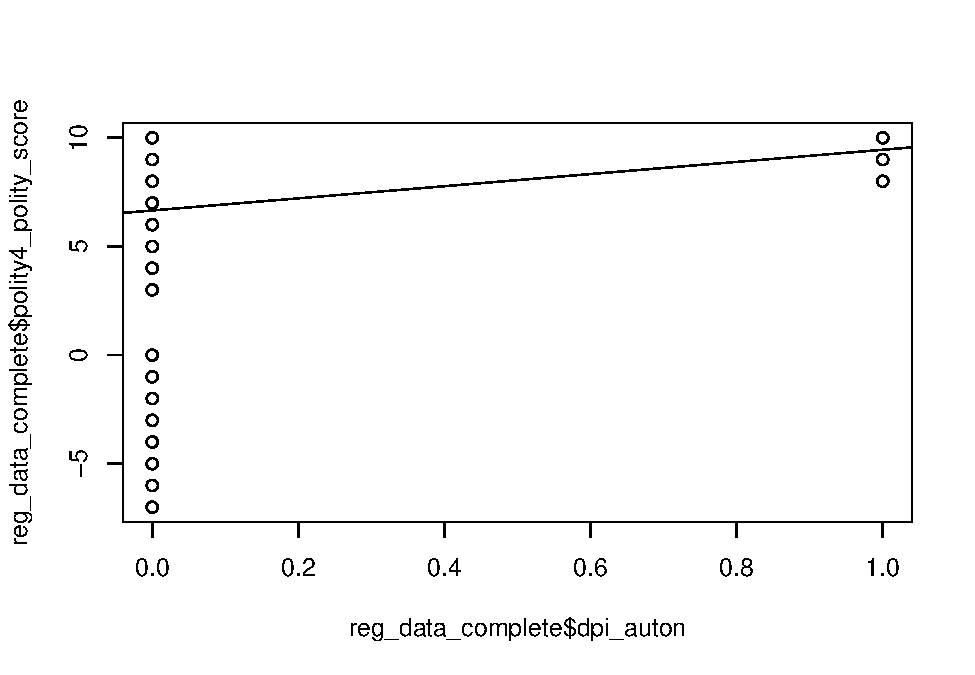
\includegraphics{05_tjbrailey_summary_statistics_files/figure-latex/unnamed-chunk-4-1.pdf}

\begin{Shaded}
\begin{Highlighting}[]
\NormalTok{reg2 <-}\StringTok{ }\KeywordTok{lm}\NormalTok{(polity4_polity_score }\OperatorTok{~}\StringTok{ }\NormalTok{idc_subtax, }\DataTypeTok{data =}\NormalTok{ reg_data_complete)}
\NormalTok{reg2_tex <-}\StringTok{ }\NormalTok{texreg}\OperatorTok{::}\KeywordTok{texreg}\NormalTok{(reg2, }\DataTypeTok{include.ci =} \OtherTok{FALSE}\NormalTok{)}
\NormalTok{reg2_tex}
\end{Highlighting}
\end{Shaded}

\begin{verbatim}
## 
## \begin{table}
## \begin{center}
## \begin{tabular}{l c}
## \hline
##  & Model 1 \\
## \hline
## (Intercept) & $5.97^{***}$ \\
##             & $(0.21)$     \\
## idc\_subtax & $2.32^{***}$ \\
##             & $(0.29)$     \\
## \hline
## R$^2$       & $0.06$       \\
## Adj. R$^2$  & $0.06$       \\
## Num. obs.   & $922$        \\
## \hline
## \multicolumn{2}{l}{\scriptsize{$^{***}p<0.001$; $^{**}p<0.01$; $^{*}p<0.05$}}
## \end{tabular}
## \caption{Statistical models}
## \label{table:coefficients}
## \end{center}
## \end{table}
\end{verbatim}

\begin{Shaded}
\begin{Highlighting}[]
\KeywordTok{plot}\NormalTok{(}\DataTypeTok{x =}\NormalTok{ reg_data_complete}\OperatorTok{$}\NormalTok{idc_subtax, }\DataTypeTok{y =}\NormalTok{ reg_data_complete}\OperatorTok{$}\NormalTok{polity4_polity_score)}
\KeywordTok{abline}\NormalTok{(}\DataTypeTok{reg =}\NormalTok{ reg2)}
\end{Highlighting}
\end{Shaded}

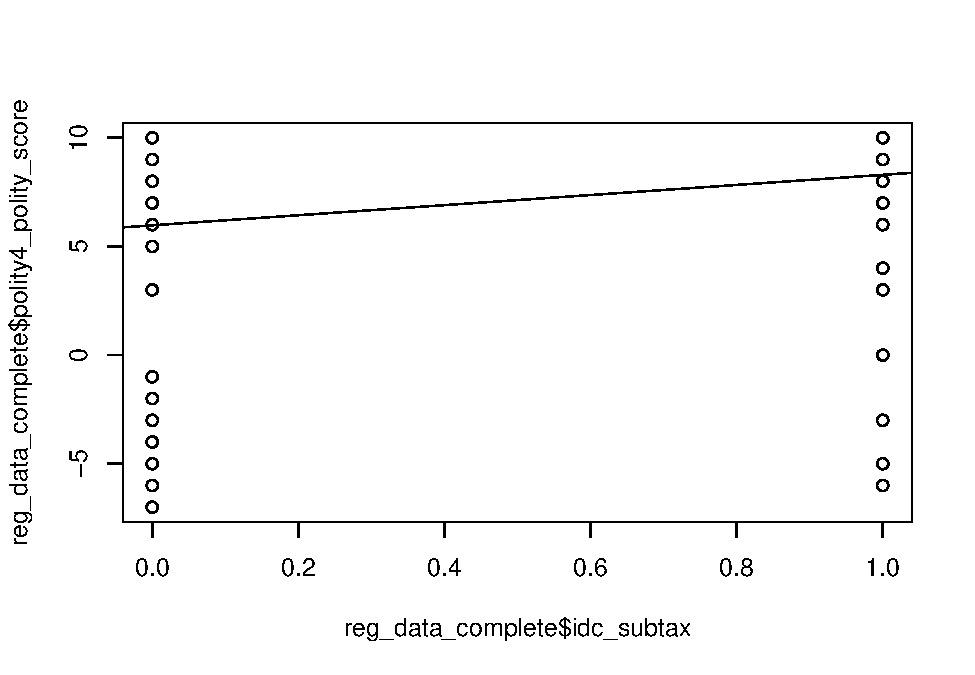
\includegraphics{05_tjbrailey_summary_statistics_files/figure-latex/unnamed-chunk-4-2.pdf}

\begin{Shaded}
\begin{Highlighting}[]
\NormalTok{reg3 <-}\StringTok{ }\KeywordTok{lm}\NormalTok{(polity4_polity_score }\OperatorTok{~}\StringTok{ }\NormalTok{idc_subed, }\DataTypeTok{data =}\NormalTok{ reg_data_complete)}
\NormalTok{reg3_tex <-}\StringTok{ }\NormalTok{texreg}\OperatorTok{::}\KeywordTok{texreg}\NormalTok{(reg3, }\DataTypeTok{include.ci =} \OtherTok{FALSE}\NormalTok{)}
\NormalTok{reg3_tex}
\end{Highlighting}
\end{Shaded}

\begin{verbatim}
## 
## \begin{table}
## \begin{center}
## \begin{tabular}{l c}
## \hline
##  & Model 1 \\
## \hline
## (Intercept) & $6.84^{***}$ \\
##             & $(0.25)$     \\
## idc\_subed  & $0.51$       \\
##             & $(0.31)$     \\
## \hline
## R$^2$       & $0.00$       \\
## Adj. R$^2$  & $0.00$       \\
## Num. obs.   & $922$        \\
## \hline
## \multicolumn{2}{l}{\scriptsize{$^{***}p<0.001$; $^{**}p<0.01$; $^{*}p<0.05$}}
## \end{tabular}
## \caption{Statistical models}
## \label{table:coefficients}
## \end{center}
## \end{table}
\end{verbatim}

\begin{Shaded}
\begin{Highlighting}[]
\KeywordTok{plot}\NormalTok{(}\DataTypeTok{x =}\NormalTok{ reg_data_complete}\OperatorTok{$}\NormalTok{idc_subed, }\DataTypeTok{y =}\NormalTok{ reg_data_complete}\OperatorTok{$}\NormalTok{polity4_polity_score)}
\KeywordTok{abline}\NormalTok{(}\DataTypeTok{reg =}\NormalTok{ reg3)}
\end{Highlighting}
\end{Shaded}

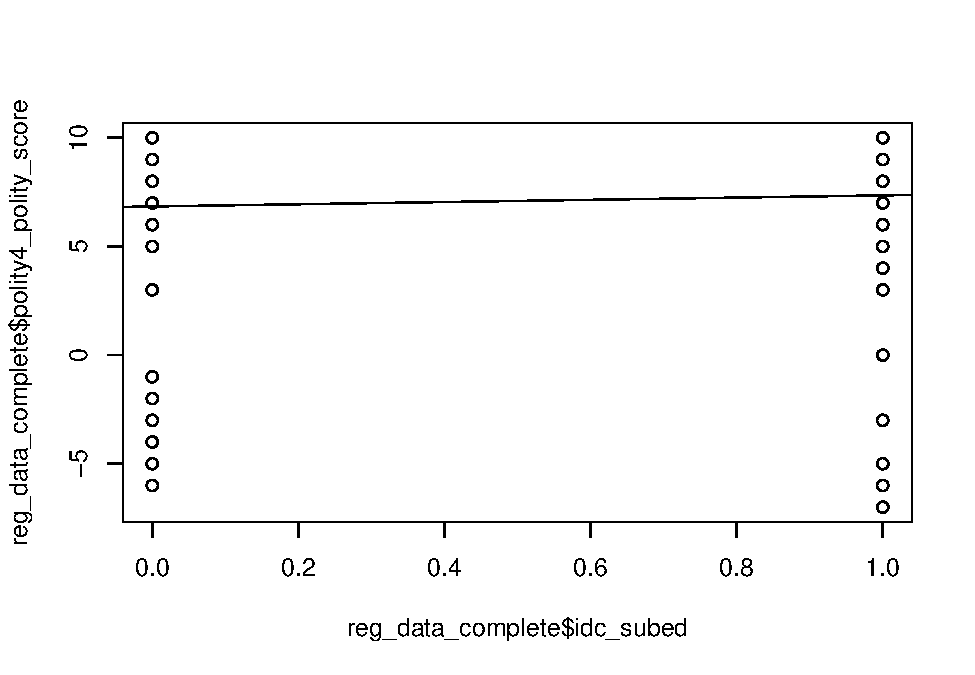
\includegraphics{05_tjbrailey_summary_statistics_files/figure-latex/unnamed-chunk-4-3.pdf}

\begin{Shaded}
\begin{Highlighting}[]
\NormalTok{reg4 <-}\StringTok{ }\KeywordTok{lm}\NormalTok{(polity4_polity_score }\OperatorTok{~}\StringTok{ }\NormalTok{idc_subpolice, }\DataTypeTok{data =}\NormalTok{ reg_data_complete)}
\NormalTok{reg4_tex <-}\StringTok{ }\NormalTok{texreg}\OperatorTok{::}\KeywordTok{texreg}\NormalTok{(reg4, }\DataTypeTok{include.ci =} \OtherTok{FALSE}\NormalTok{)}
\NormalTok{reg4_tex}
\end{Highlighting}
\end{Shaded}

\begin{verbatim}
## 
## \begin{table}
## \begin{center}
## \begin{tabular}{l c}
## \hline
##  & Model 1 \\
## \hline
## (Intercept)    & $5.95^{***}$ \\
##                & $(0.20)$     \\
## idc\_subpolice & $2.46^{***}$ \\
##                & $(0.29)$     \\
## \hline
## R$^2$          & $0.07$       \\
## Adj. R$^2$     & $0.07$       \\
## Num. obs.      & $922$        \\
## \hline
## \multicolumn{2}{l}{\scriptsize{$^{***}p<0.001$; $^{**}p<0.01$; $^{*}p<0.05$}}
## \end{tabular}
## \caption{Statistical models}
## \label{table:coefficients}
## \end{center}
## \end{table}
\end{verbatim}

\begin{Shaded}
\begin{Highlighting}[]
\KeywordTok{plot}\NormalTok{(}\DataTypeTok{x =}\NormalTok{ reg_data_complete}\OperatorTok{$}\NormalTok{idc_subpolice, }\DataTypeTok{y =}\NormalTok{ reg_data_complete}\OperatorTok{$}\NormalTok{polity4_polity_score)}
\KeywordTok{abline}\NormalTok{(}\DataTypeTok{reg =}\NormalTok{ reg4)}
\end{Highlighting}
\end{Shaded}

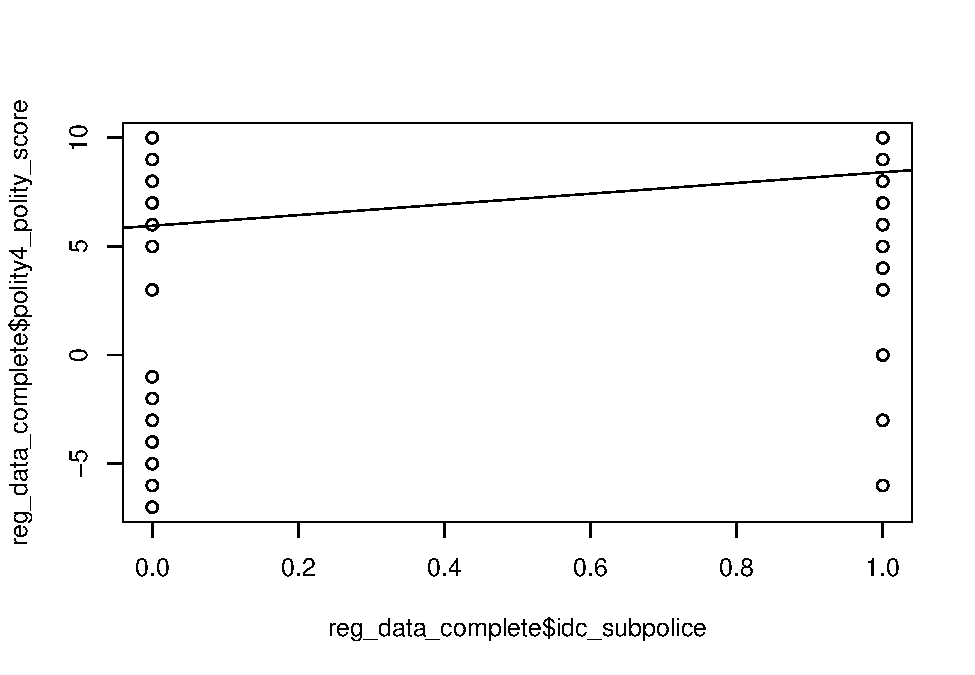
\includegraphics{05_tjbrailey_summary_statistics_files/figure-latex/unnamed-chunk-4-4.pdf}

\begin{Shaded}
\begin{Highlighting}[]
\NormalTok{reg5 <-}\StringTok{ }\KeywordTok{lm}\NormalTok{(polity4_polity_score }\OperatorTok{~}\StringTok{ }\NormalTok{n_RAI, }\DataTypeTok{data =}\NormalTok{ reg_data_complete)}
\NormalTok{reg5_tex <-}\StringTok{ }\NormalTok{texreg}\OperatorTok{::}\KeywordTok{texreg}\NormalTok{(reg5, }\DataTypeTok{include.ci =} \OtherTok{FALSE}\NormalTok{)}
\NormalTok{reg5_tex}
\end{Highlighting}
\end{Shaded}

\begin{verbatim}
## 
## \begin{table}
## \begin{center}
## \begin{tabular}{l c}
## \hline
##  & Model 1 \\
## \hline
## (Intercept) & $5.31^{***}$ \\
##             & $(0.22)$     \\
## n\_RAI      & $0.13^{***}$ \\
##             & $(0.01)$     \\
## \hline
## R$^2$       & $0.11$       \\
## Adj. R$^2$  & $0.11$       \\
## Num. obs.   & $922$        \\
## \hline
## \multicolumn{2}{l}{\scriptsize{$^{***}p<0.001$; $^{**}p<0.01$; $^{*}p<0.05$}}
## \end{tabular}
## \caption{Statistical models}
## \label{table:coefficients}
## \end{center}
## \end{table}
\end{verbatim}

\begin{Shaded}
\begin{Highlighting}[]
\KeywordTok{jpeg}\NormalTok{(}\DataTypeTok{filename =} \KeywordTok{paste0}\NormalTok{(here}\OperatorTok{::}\KeywordTok{here}\NormalTok{(), }\StringTok{"/vis/polity_score_rai_reg.jpeg"}\NormalTok{))}
\KeywordTok{plot}\NormalTok{(}\DataTypeTok{x =}\NormalTok{ reg_data_complete}\OperatorTok{$}\NormalTok{n_RAI, }
     \DataTypeTok{y =}\NormalTok{ reg_data_complete}\OperatorTok{$}\NormalTok{polity4_polity_score,}
     \DataTypeTok{xlab =} \StringTok{"RAI Measure of Autonomy"}\NormalTok{, }
     \DataTypeTok{ylab =} \StringTok{"Polity Score"}\NormalTok{, }
     \DataTypeTok{main =} \StringTok{"Predicting Polity Score with Regional Autonomy Provisions"}\NormalTok{)}
\KeywordTok{abline}\NormalTok{(}\DataTypeTok{reg =}\NormalTok{ reg5, }\DataTypeTok{col =} \StringTok{"red"}\NormalTok{)}
\KeywordTok{dev.off}\NormalTok{()}
\end{Highlighting}
\end{Shaded}

\begin{verbatim}
## pdf 
##   2
\end{verbatim}

\begin{Shaded}
\begin{Highlighting}[]
\NormalTok{reg6 <-}\StringTok{ }\KeywordTok{lm}\NormalTok{(polity4_polity_score }\OperatorTok{~}\StringTok{ }\NormalTok{reg_aut_dum, }\DataTypeTok{data =}\NormalTok{ reg_data_complete)}
\NormalTok{reg6_tex <-}\StringTok{ }\NormalTok{texreg}\OperatorTok{::}\KeywordTok{texreg}\NormalTok{(reg6, }\DataTypeTok{include.ci =} \OtherTok{FALSE}\NormalTok{)}
\NormalTok{reg6_tex}
\end{Highlighting}
\end{Shaded}

\begin{verbatim}
## 
## \begin{table}
## \begin{center}
## \begin{tabular}{l c}
## \hline
##  & Model 1 \\
## \hline
## (Intercept)       & $6.42^{***}$ \\
##                   & $(0.18)$     \\
## reg\_aut\_dumTRUE & $2.12^{***}$ \\
##                   & $(0.31)$     \\
## \hline
## R$^2$             & $0.05$       \\
## Adj. R$^2$        & $0.05$       \\
## Num. obs.         & $922$        \\
## \hline
## \multicolumn{2}{l}{\scriptsize{$^{***}p<0.001$; $^{**}p<0.01$; $^{*}p<0.05$}}
## \end{tabular}
## \caption{Statistical models}
## \label{table:coefficients}
## \end{center}
## \end{table}
\end{verbatim}

\begin{Shaded}
\begin{Highlighting}[]
\KeywordTok{plot}\NormalTok{(}\DataTypeTok{x =}\NormalTok{ reg_data_complete}\OperatorTok{$}\NormalTok{reg_aut_dum, }\DataTypeTok{y =}\NormalTok{ reg_data_complete}\OperatorTok{$}\NormalTok{polity4_polity_score)}
\KeywordTok{abline}\NormalTok{(}\DataTypeTok{reg =}\NormalTok{ reg6)}
\end{Highlighting}
\end{Shaded}

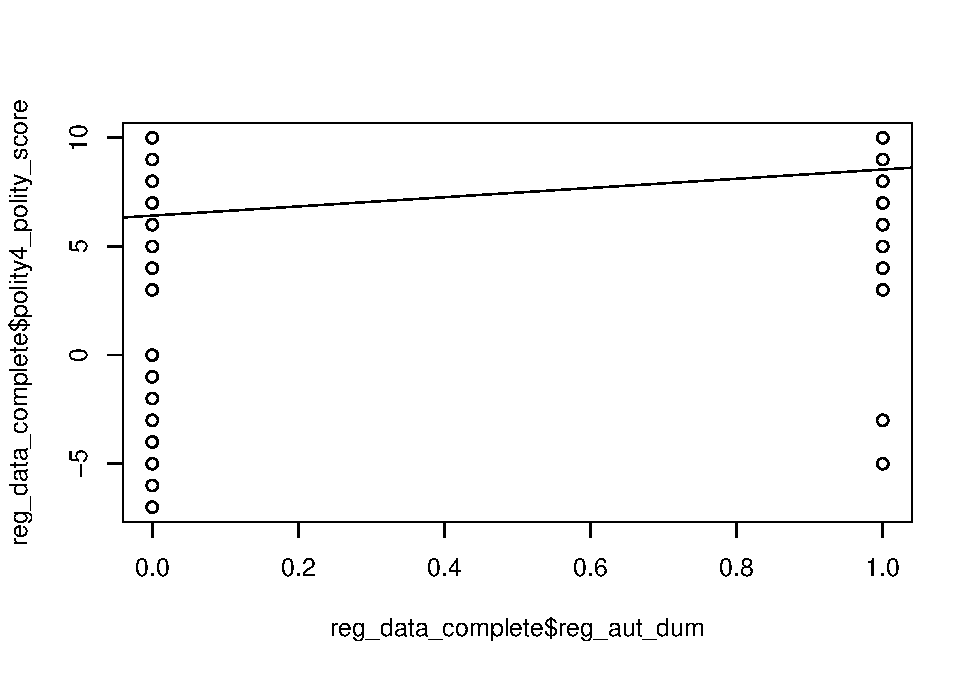
\includegraphics{05_tjbrailey_summary_statistics_files/figure-latex/unnamed-chunk-4-5.pdf}

\begin{Shaded}
\begin{Highlighting}[]
\NormalTok{reg_full_tex <-}\StringTok{ }\NormalTok{texreg}\OperatorTok{::}\KeywordTok{texreg}\NormalTok{(}\KeywordTok{list}\NormalTok{(reg1, reg5, reg6), }
                              \DataTypeTok{mfrow =} \OtherTok{TRUE}\NormalTok{, }
                              \DataTypeTok{omit.coef =} \StringTok{"as.factor"}\NormalTok{, }
                              \DataTypeTok{include.ci =} \OtherTok{FALSE}\NormalTok{) }

\NormalTok{reg_full_tex}
\end{Highlighting}
\end{Shaded}

\begin{verbatim}
## 
## \begin{table}
## \begin{center}
## \begin{tabular}{l c c c}
## \hline
##  & Model 1 & Model 2 & Model 3 \\
## \hline
## (Intercept)       & $6.65^{***}$ & $5.31^{***}$ & $6.42^{***}$ \\
##                   & $(0.16)$     & $(0.22)$     & $(0.18)$     \\
## dpi\_autonTRUE    & $2.79^{***}$ &              &              \\
##                   & $(0.38)$     &              &              \\
## n\_RAI            &              & $0.13^{***}$ &              \\
##                   &              & $(0.01)$     &              \\
## reg\_aut\_dumTRUE &              &              & $2.12^{***}$ \\
##                   &              &              & $(0.31)$     \\
## \hline
## R$^2$             & $0.06$       & $0.11$       & $0.05$       \\
## Adj. R$^2$        & $0.05$       & $0.11$       & $0.05$       \\
## Num. obs.         & $922$        & $922$        & $922$        \\
## \hline
## \multicolumn{4}{l}{\scriptsize{$^{***}p<0.001$; $^{**}p<0.01$; $^{*}p<0.05$}}
## \end{tabular}
## \caption{Statistical models}
## \label{table:coefficients}
## \end{center}
## \end{table}
\end{verbatim}

\end{document}
